\documentclass[]{book}
\usepackage{lmodern}
\usepackage{amssymb,amsmath}
\usepackage{ifxetex,ifluatex}
\usepackage{fixltx2e} % provides \textsubscript
\ifnum 0\ifxetex 1\fi\ifluatex 1\fi=0 % if pdftex
  \usepackage[T1]{fontenc}
  \usepackage[utf8]{inputenc}
\else % if luatex or xelatex
  \ifxetex
    \usepackage{mathspec}
  \else
    \usepackage{fontspec}
  \fi
  \defaultfontfeatures{Ligatures=TeX,Scale=MatchLowercase}
\fi
% use upquote if available, for straight quotes in verbatim environments
\IfFileExists{upquote.sty}{\usepackage{upquote}}{}
% use microtype if available
\IfFileExists{microtype.sty}{%
\usepackage{microtype}
\UseMicrotypeSet[protrusion]{basicmath} % disable protrusion for tt fonts
}{}
\usepackage[margin=1in]{geometry}
\usepackage{hyperref}
\hypersetup{unicode=true,
            pdftitle={Neural Network and Deep Learning},
            pdfauthor={Guang Yang},
            pdfborder={0 0 0},
            breaklinks=true}
\urlstyle{same}  % don't use monospace font for urls
\usepackage{natbib}
\bibliographystyle{apalike}
\usepackage{color}
\usepackage{fancyvrb}
\newcommand{\VerbBar}{|}
\newcommand{\VERB}{\Verb[commandchars=\\\{\}]}
\DefineVerbatimEnvironment{Highlighting}{Verbatim}{commandchars=\\\{\}}
% Add ',fontsize=\small' for more characters per line
\usepackage{framed}
\definecolor{shadecolor}{RGB}{248,248,248}
\newenvironment{Shaded}{\begin{snugshade}}{\end{snugshade}}
\newcommand{\KeywordTok}[1]{\textcolor[rgb]{0.13,0.29,0.53}{\textbf{{#1}}}}
\newcommand{\DataTypeTok}[1]{\textcolor[rgb]{0.13,0.29,0.53}{{#1}}}
\newcommand{\DecValTok}[1]{\textcolor[rgb]{0.00,0.00,0.81}{{#1}}}
\newcommand{\BaseNTok}[1]{\textcolor[rgb]{0.00,0.00,0.81}{{#1}}}
\newcommand{\FloatTok}[1]{\textcolor[rgb]{0.00,0.00,0.81}{{#1}}}
\newcommand{\ConstantTok}[1]{\textcolor[rgb]{0.00,0.00,0.00}{{#1}}}
\newcommand{\CharTok}[1]{\textcolor[rgb]{0.31,0.60,0.02}{{#1}}}
\newcommand{\SpecialCharTok}[1]{\textcolor[rgb]{0.00,0.00,0.00}{{#1}}}
\newcommand{\StringTok}[1]{\textcolor[rgb]{0.31,0.60,0.02}{{#1}}}
\newcommand{\VerbatimStringTok}[1]{\textcolor[rgb]{0.31,0.60,0.02}{{#1}}}
\newcommand{\SpecialStringTok}[1]{\textcolor[rgb]{0.31,0.60,0.02}{{#1}}}
\newcommand{\ImportTok}[1]{{#1}}
\newcommand{\CommentTok}[1]{\textcolor[rgb]{0.56,0.35,0.01}{\textit{{#1}}}}
\newcommand{\DocumentationTok}[1]{\textcolor[rgb]{0.56,0.35,0.01}{\textbf{\textit{{#1}}}}}
\newcommand{\AnnotationTok}[1]{\textcolor[rgb]{0.56,0.35,0.01}{\textbf{\textit{{#1}}}}}
\newcommand{\CommentVarTok}[1]{\textcolor[rgb]{0.56,0.35,0.01}{\textbf{\textit{{#1}}}}}
\newcommand{\OtherTok}[1]{\textcolor[rgb]{0.56,0.35,0.01}{{#1}}}
\newcommand{\FunctionTok}[1]{\textcolor[rgb]{0.00,0.00,0.00}{{#1}}}
\newcommand{\VariableTok}[1]{\textcolor[rgb]{0.00,0.00,0.00}{{#1}}}
\newcommand{\ControlFlowTok}[1]{\textcolor[rgb]{0.13,0.29,0.53}{\textbf{{#1}}}}
\newcommand{\OperatorTok}[1]{\textcolor[rgb]{0.81,0.36,0.00}{\textbf{{#1}}}}
\newcommand{\BuiltInTok}[1]{{#1}}
\newcommand{\ExtensionTok}[1]{{#1}}
\newcommand{\PreprocessorTok}[1]{\textcolor[rgb]{0.56,0.35,0.01}{\textit{{#1}}}}
\newcommand{\AttributeTok}[1]{\textcolor[rgb]{0.77,0.63,0.00}{{#1}}}
\newcommand{\RegionMarkerTok}[1]{{#1}}
\newcommand{\InformationTok}[1]{\textcolor[rgb]{0.56,0.35,0.01}{\textbf{\textit{{#1}}}}}
\newcommand{\WarningTok}[1]{\textcolor[rgb]{0.56,0.35,0.01}{\textbf{\textit{{#1}}}}}
\newcommand{\AlertTok}[1]{\textcolor[rgb]{0.94,0.16,0.16}{{#1}}}
\newcommand{\ErrorTok}[1]{\textcolor[rgb]{0.64,0.00,0.00}{\textbf{{#1}}}}
\newcommand{\NormalTok}[1]{{#1}}
\usepackage{longtable,booktabs}
\usepackage{graphicx,grffile}
\makeatletter
\def\maxwidth{\ifdim\Gin@nat@width>\linewidth\linewidth\else\Gin@nat@width\fi}
\def\maxheight{\ifdim\Gin@nat@height>\textheight\textheight\else\Gin@nat@height\fi}
\makeatother
% Scale images if necessary, so that they will not overflow the page
% margins by default, and it is still possible to overwrite the defaults
% using explicit options in \includegraphics[width, height, ...]{}
\setkeys{Gin}{width=\maxwidth,height=\maxheight,keepaspectratio}
\IfFileExists{parskip.sty}{%
\usepackage{parskip}
}{% else
\setlength{\parindent}{0pt}
\setlength{\parskip}{6pt plus 2pt minus 1pt}
}
\setlength{\emergencystretch}{3em}  % prevent overfull lines
\providecommand{\tightlist}{%
  \setlength{\itemsep}{0pt}\setlength{\parskip}{0pt}}
\setcounter{secnumdepth}{5}
% Redefines (sub)paragraphs to behave more like sections
\ifx\paragraph\undefined\else
\let\oldparagraph\paragraph
\renewcommand{\paragraph}[1]{\oldparagraph{#1}\mbox{}}
\fi
\ifx\subparagraph\undefined\else
\let\oldsubparagraph\subparagraph
\renewcommand{\subparagraph}[1]{\oldsubparagraph{#1}\mbox{}}
\fi

%%% Use protect on footnotes to avoid problems with footnotes in titles
\let\rmarkdownfootnote\footnote%
\def\footnote{\protect\rmarkdownfootnote}

%%% Change title format to be more compact
\usepackage{titling}

% Create subtitle command for use in maketitle
\newcommand{\subtitle}[1]{
  \posttitle{
    \begin{center}\large#1\end{center}
    }
}

\setlength{\droptitle}{-2em}
  \title{Neural Network and Deep Learning}
  \pretitle{\vspace{\droptitle}\centering\huge}
  \posttitle{\par}
  \author{Guang Yang}
  \preauthor{\centering\large\emph}
  \postauthor{\par}
  \predate{\centering\large\emph}
  \postdate{\par}
  \date{2016-12-09}

\usepackage{booktabs}

\begin{document}
\maketitle

{
\setcounter{tocdepth}{1}
\tableofcontents
}
\chapter*{Preface}\label{preface}
\addcontentsline{toc}{chapter}{Preface}

\textbf{Welcome \ldots{}}

\chapter{Using neural network to recognize handwritten
digits}\label{nnhd}

\section{Perceptrons}\label{perceptrons}

A perceptron makes decisions by weighing up evidence - a perceptron
receives several \textbf{binary inputs}, \(x_1, x_2, ...\) and produces
a single \textbf{binary output}:

\begin{figure}

{\centering 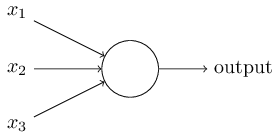
\includegraphics[width=0.3\linewidth]{fig/01_tikz00} 

}

\caption{Perceptrons}\label{fig:nnhd-pptn}
\end{figure}

In math:

\begin{equation}
\mbox{output} = \left\{ 
  \begin{array}{ll} 
    0 & \mbox{if } w\cdot x + b \leq 0 \\
    1 & \mbox{if } w\cdot x + b > 0
  \end{array}
\right.
\label{eq:nnhd-pptn}
\end{equation}

In equation \eqref{eq:nnhd-pptn}, \(b\) is called bias - a measure of how
easy it is to get the perceptron to output a 1. Or to put it in more
biological terms, the bias is a measure of how easy it is to get the
perceptron to \textbf{fire}.

Perceptrons can together built to a multi-layer decision making system:

\begin{figure}

{\centering 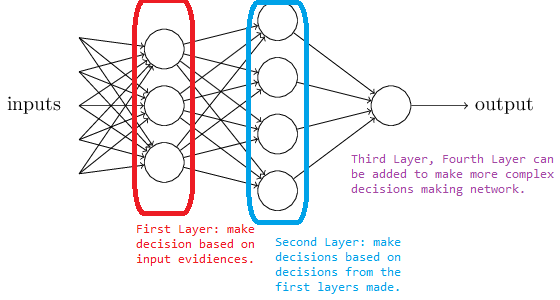
\includegraphics[width=0.75\linewidth]{fig/01_tikz01} 

}

\caption{Perceptrons can together built to a multi-layer decision making system.}\label{fig:nnhd-pptm}
\end{figure}

Perceptrons can realize elementary logical functions such as
\texttt{AND}, \texttt{OR} and \texttt{NAND}. The \texttt{NAND} gate is
significant because any boolean function can be implemented by using a
combination of \texttt{NAND} gates. This property is called
\textbf{functional completeness}. It follows that perceptrons are also
universal for computation.

\begin{figure}

{\centering 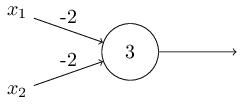
\includegraphics[width=0.4\linewidth]{fig/01_tikz02} 

}

\caption{Perceptrons realize NAND gate.}\label{fig:nnhd-pptn-nand}
\end{figure}

Example: use NAND gates and repeatedly perceptrons to build a circuit
which adds two bits, \(x_1\) and \(x_2\) by computing the bitwise sum,
\(x_1\) ⊕ \(x_2\), as well as a carry bit which is set to 1 when both
\(x_1\) and \(x_2\) are 1, i.e., the carry bit is just the bitwise
product \(x_1x_2\):

\begin{figure}

{\centering 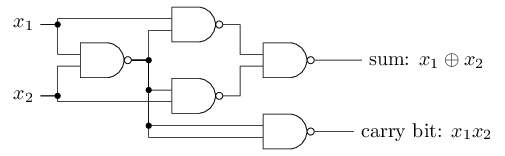
\includegraphics[width=0.5\linewidth]{fig/01_tikz03} 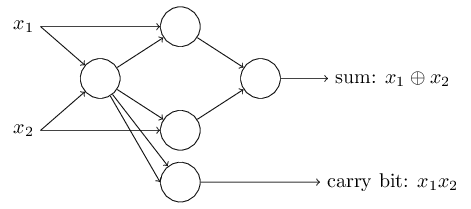
\includegraphics[width=0.5\linewidth]{fig/01_tikz04} 

}

\caption{Perceptrons and NAND gate implementation of sum.}\label{fig:nnhd-pptn-nand-sum}
\end{figure}

\section{Sigmoid Neuron}\label{sigmoid-neuron}

\textbf{Motivation from Perceptrons to Sigmoid Neuron}: The desire of a
small change in a weight (or bias) causes only a small change in output,
so that modify the weights and biases gradually can make the network
getting closer and closer to the desired behaviour.

\begin{figure}

{\centering 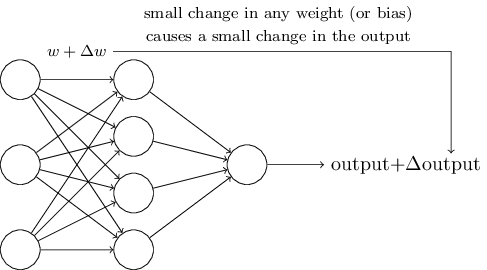
\includegraphics[width=0.7\linewidth]{fig/01_tikz08} 

}

\caption{Motivation of using Sigmoid Neuron.}\label{fig:nnhd-sn-motivation}
\end{figure}

Sigmoid neurons are similar to perceptrons, but modified so that small
changes in their weights and bias cause only a small change in their
output. A sigmoid neuron receives inputs of \textbf{values between 0 and
1}, and produces output of a \textbf{value between 0 and 1}, via the
\textbf{sigmoid function}:

\begin{equation} 
\sigma(z) \equiv \frac{1}{1 + e^{-z}} = \frac{1}{1 + \exp(-\sum_j w_j x_j - b)}.
\label{eq:nnhd-sn-sigmoid}
\end{equation}

The smoothness of \(\sigma\) means that small changes \(\Delta w_j\) in
the weights and \(\Delta b\) in the bias will produce a small change
\(\Delta \mbox{output}\) in the output from the neuron, where

\begin{equation} 
\Delta \mbox{output} \approx \sum_j \frac{\partial \, \mbox{output}}{\partial w_j} \Delta w_j + 
                             \frac{\partial \, \mbox{output}}{\partial b} \Delta b,
\label{eq:nnhd-sn-smoothness}
\end{equation}

is the sum over all the changes in weights \(w_j\) and bias \(b\),
weighted by the partial derivatives of the output to \(w_j\) and \(b\),
respectively.

\section{The architecture of neural
networks}\label{the-architecture-of-neural-networks}

\begin{figure}

{\centering 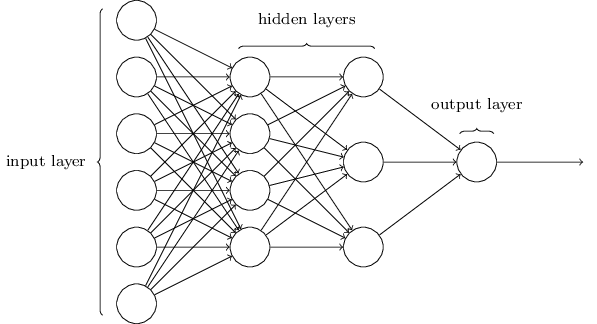
\includegraphics[width=0.7\linewidth]{fig/01_tikz11} 

}

\caption{The Architecture of Neural Networks.}\label{fig:nnhd-nn-architecture}
\end{figure}

\textbf{Feedforward neural networks}: no loops in the network -
information is always fed forward, never fed back.

\textbf{Recurrent neural networks}: The idea in these models is to have
neurons which fire for some limited duration of time, before becoming
quiescent. That firing can stimulate other neurons, which may fire a
little while later, also for a limited duration. That causes still more
neurons to fire, and so over time we get a cascade of neurons firing.
Loops don't cause problems in such a model, since a neuron's output only
affects its input at some later time, not instantaneously. Hard to
train, but closer to the spirit to how human brains work.

\section{A simple network to classify handwritten
digits}\label{a-simple-network-to-classify-handwritten-digits}

\begin{figure}

{\centering 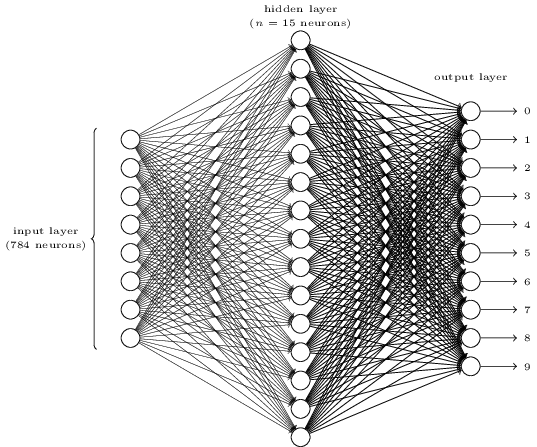
\includegraphics[width=0.7\linewidth]{fig/01_tikz12} 

}

\caption{The three layer neural networks for recognizing individual digits.}\label{fig:nnhd-nn-digit}
\end{figure}

\section{Learning with gradient
descent}\label{learning-with-gradient-descent}

\subsection{Init}\label{init}

\begin{itemize}
\item
  Training and Testing Data: MNIST dataset - split 60000 training images
  into 50000 training and 10000 validating for hyper-parameters such as
  learning rate, with 10000 testing images kept still.
\item
  Output: \(y = y(x)\) a 10-dimensional indicator vector.
\item
  Cost Function, a.k.a, Loss Function, Objective Function:
\end{itemize}

\begin{equation}  
C(w,b) \equiv \frac{1}{2n} \sum_x \| y(x) - a\|^2.
\label{eq:nnhd-gd-cf}
\end{equation}

\subsection{The gradient descent method as an optimization
approach}\label{the-gradient-descent-method-as-an-optimization-approach}

\subsubsection{The gradient descent
method}\label{the-gradient-descent-method}

Consider minimizing any function \(C(v), v = v_1, v_2, \ldots, v_m\),
known that

\begin{equation} 
\Delta C \approx \frac{\partial C}{\partial v_1} \Delta v_1 + 
                 \frac{\partial C}{\partial v_2} \Delta v_2 +
                 \cdots
                 \frac{\partial C}{\partial v_m} \Delta v_m +
         = \nabla C \cdot \Delta v.
\label{eq:nnhd-gd-1d}
\end{equation}

where
\(\displaystyle \nabla C \equiv \left(\frac{\partial C}{\partial v_1}, \ldots, \frac{\partial C}{\partial v_m}\right)^T\)
is the \textbf{gradient} of \(C\), then choose

\begin{equation} 
\Delta v = -\eta \nabla C,
\label{eq:nnhd-gd-dc}
\end{equation}

with a small positive \textbf{learning rate} \(\eta\) means
\(\displaystyle \Delta C \approx -\eta \nabla C \cdot \nabla C = -\eta \|\nabla C\|^2\)
is negative guaranteed, e.g., makes \(C\) montonically decreasing.

Thus, Equation \eqref{eq:nnhd-gd-dc} defines the \textbf{law of motion},
and suggests searching parameters \(v\) by

\begin{equation}
v \rightarrow v' = v -\eta \nabla C.
\label{eq:nnhd-gd-mv}
\end{equation}

repeatedly for minimizing \(C\).

An alternative view on Equation \eqref{eq:nnhd-gd-mv} is that it defines
the choice \(\Delta v\) which minimizes \(\nabla C \cdot \Delta v\) by
taking \(\eta = \epsilon / \|\nabla C\|\) when
\(\|\Delta v\| = \epsilon\) is fixed - gradient descent can be viewed as
a way of taking small steps in the direction which does the most to
immediately decrease \(C\).

In summary, the gradient descent algorithm computes the gradient
\(\nabla C\), and then moves a small step to the opposite direction of
gradient, repeatedly.

\subsubsection{Apply gradient descent to learn in a neural
network}\label{apply-gradient-descent-to-learn-in-a-neural-network}

In general, instance \(v\) with \(w\) and \(b\), such as updating

\begin{equation}
\begin{array}{rcccl}
w_k & \rightarrow & w_k' & = & w_k-\eta \frac{\partial C}{\partial w_k} \\
b_l & \rightarrow & b_l' & = & b_l-\eta \frac{\partial C}{\partial b_l}.
\end{array}\label{eq:nnhd-gd-mw}
\end{equation}

Take advantage that cost function has structure
\(\displaystyle C = \frac{1}{n} \sum_x C_x\) average over costs
\(\displaystyle C_x \equiv \frac{\|y(x)-a\|^2}{2}\), \textbf{stochastic
gradient descent} speeds up learning by estimating the gradient
\(\nabla C\) by computing \(\nabla C_x\) for a small sample of randomly
chosen training inputs called min-batch.

Speaking explicitly, suppose \(w_k\) and \(b_l\) denote the weights and
biases in our neural network. Then stochastic gradient descent picks a
randomly chosen mini-batch of training inputs, and training with those,

\begin{equation}
\begin{array}{rcccl}
w_k & \rightarrow & w_k' & = & w_k-\frac{\eta}{m} \sum_j \frac{\partial C_{X_j}}{\partial w_k} \\
b_l & \rightarrow & b_l' & = & b_l-\frac{\eta}{m} \sum_j \frac{\partial C_{X_j}}{\partial b_l}.
\end{array}\label{eq:nnhd-sgd-mw}
\end{equation}

where the sums are over all the training examples \(X_j\) in the current
mini-batch. Then pick out another randomly chosen mini-batch and train
with those. And so on, until exhaust the training inputs, which is said
to complete an \textbf{epoch} of training. At that point, start over
with a new training epoch.

An extreme case is to use a size 1 mini-batch, a.k.a, \textbf{online},
\textbf{on-line} or \textbf{incremental} learning.

\subsection{Solver}\label{solver}

See code and note on \texttt{network.py} and \texttt{network\_note.py}
in \href{./src}{source code folder}.

\begin{Shaded}
\begin{Highlighting}[]
\CommentTok{"""}
\CommentTok{network.py}
\CommentTok{~~~~~~~~~~}

\CommentTok{A module to implement the stochastic gradient descent learning algorithm for a }
\CommentTok{feedforward neural network.  Gradients are calculated using backpropagation.  }
\CommentTok{Note that I have focused on making the code simple, easily readable, and easily}
\CommentTok{modifiable.  It is not optimized, and omits many desirable features.}
\CommentTok{"""}

\CommentTok{#### Libraries}
\CommentTok{# Standard library}
\ImportTok{import} \NormalTok{random}

\CommentTok{# Third-party libraries}
\ImportTok{import} \NormalTok{numpy }\ImportTok{as} \NormalTok{np}

\KeywordTok{class} \NormalTok{Network(}\BuiltInTok{object}\NormalTok{):}

    \KeywordTok{def} \FunctionTok{__init__}\NormalTok{(}\VariableTok{self}\NormalTok{, sizes):}
        \CommentTok{"""The list ``sizes`` contains the number of neurons in the respective }
\CommentTok{        layers of the network.  For example, if the list was [2, 3, 1] then it}
\CommentTok{        would be a three-layer network, with the first layer containing 2 }
\CommentTok{        neurons, the second layer 3 neurons, and the third layer 1 neuron.  }
\CommentTok{        The biases and weights for the network are initialized randomly, using }
\CommentTok{        a Gaussian distribution with mean 0, and variance 1.  Note that the }
\CommentTok{        first layer is assumed to be an input layer, and by convention we won't }
\CommentTok{        set any biases for those neurons, since biases are only ever used in }
\CommentTok{        computing the outputs from later layers."""}
        \VariableTok{self}\NormalTok{.num_layers }\OperatorTok{=} \BuiltInTok{len}\NormalTok{(sizes)}
        \VariableTok{self}\NormalTok{.sizes }\OperatorTok{=} \NormalTok{sizes}
        \VariableTok{self}\NormalTok{.biases }\OperatorTok{=} \NormalTok{[np.random.randn(y, }\DecValTok{1}\NormalTok{) }\ControlFlowTok{for} \NormalTok{y }\OperatorTok{in} \NormalTok{sizes[}\DecValTok{1}\NormalTok{:]]}
        \VariableTok{self}\NormalTok{.weights }\OperatorTok{=} \NormalTok{[np.random.randn(y, x)}
                        \ControlFlowTok{for} \NormalTok{x, y }\OperatorTok{in} \BuiltInTok{zip}\NormalTok{(sizes[:}\OperatorTok{-}\DecValTok{1}\NormalTok{], sizes[}\DecValTok{1}\NormalTok{:])]}

    \KeywordTok{def} \NormalTok{feedforward(}\VariableTok{self}\NormalTok{, a):}
        \CommentTok{"""Return the output of the network if ``a`` is input."""}
        \ControlFlowTok{for} \NormalTok{b, w }\OperatorTok{in} \BuiltInTok{zip}\NormalTok{(}\VariableTok{self}\NormalTok{.biases, }\VariableTok{self}\NormalTok{.weights):}
            \NormalTok{a }\OperatorTok{=} \NormalTok{sigmoid(np.dot(w, a)}\OperatorTok{+}\NormalTok{b)}
        \ControlFlowTok{return} \NormalTok{a}

    \KeywordTok{def} \NormalTok{SGD(}\VariableTok{self}\NormalTok{, training_data, epochs, mini_batch_size, eta,}
            \NormalTok{test_data}\OperatorTok{=}\VariableTok{None}\NormalTok{):}
        \CommentTok{"""Train the neural network using mini-batch stochastic gradient descent.}
\CommentTok{        The ``training_data`` is a list of tuples ``(x, y)`` representing the }
\CommentTok{        training inputs and the desired outputs.  The other non-optional }
\CommentTok{        parameters are self-explanatory.  If ``test_data`` is provided then the}
\CommentTok{        network will be evaluated against the test data after each epoch, and }
\CommentTok{        partial progress printed out.  This is useful for tracking progress, }
\CommentTok{        but slows things down substantially."""}
        \ControlFlowTok{if} \NormalTok{test_data: n_test }\OperatorTok{=} \BuiltInTok{len}\NormalTok{(test_data)}
        \NormalTok{n }\OperatorTok{=} \BuiltInTok{len}\NormalTok{(training_data)}
        \ControlFlowTok{for} \NormalTok{j }\OperatorTok{in} \BuiltInTok{xrange}\NormalTok{(epochs):}
            \NormalTok{random.shuffle(training_data)}
            \NormalTok{mini_batches }\OperatorTok{=} \NormalTok{[}
                \NormalTok{training_data[k:k}\OperatorTok{+}\NormalTok{mini_batch_size]}
                \ControlFlowTok{for} \NormalTok{k }\OperatorTok{in} \BuiltInTok{xrange}\NormalTok{(}\DecValTok{0}\NormalTok{, n, mini_batch_size)]}
            \ControlFlowTok{for} \NormalTok{mini_batch }\OperatorTok{in} \NormalTok{mini_batches:}
                \VariableTok{self}\NormalTok{.update_mini_batch(mini_batch, eta)}
            \ControlFlowTok{if} \NormalTok{test_data:}
                \BuiltInTok{print} \StringTok{"Epoch }\SpecialCharTok{\{0\}}\StringTok{: }\SpecialCharTok{\{1\}}\StringTok{ / }\SpecialCharTok{\{2\}}\StringTok{"}\NormalTok{.}\BuiltInTok{format}\NormalTok{(}
                    \NormalTok{j, }\VariableTok{self}\NormalTok{.evaluate(test_data), n_test)}
            \ControlFlowTok{else}\NormalTok{:}
                \BuiltInTok{print} \StringTok{"Epoch }\SpecialCharTok{\{0\}}\StringTok{ complete"}\NormalTok{.}\BuiltInTok{format}\NormalTok{(j)}

    \KeywordTok{def} \NormalTok{update_mini_batch(}\VariableTok{self}\NormalTok{, mini_batch, eta):}
        \CommentTok{"""Update the network's weights and biases by applying gradient descent }
\CommentTok{        using backpropagation to a single mini batch.  The ``mini_batch`` is a }
\CommentTok{        list of tuples ``(x, y)``, and ``eta`` is the learning rate."""}
        \NormalTok{nabla_b }\OperatorTok{=} \NormalTok{[np.zeros(b.shape) }\ControlFlowTok{for} \NormalTok{b }\OperatorTok{in} \VariableTok{self}\NormalTok{.biases]}
        \NormalTok{nabla_w }\OperatorTok{=} \NormalTok{[np.zeros(w.shape) }\ControlFlowTok{for} \NormalTok{w }\OperatorTok{in} \VariableTok{self}\NormalTok{.weights]}
        \ControlFlowTok{for} \NormalTok{x, y }\OperatorTok{in} \NormalTok{mini_batch:}
            \NormalTok{delta_nabla_b, delta_nabla_w }\OperatorTok{=} \VariableTok{self}\NormalTok{.backprop(x, y)}
            \NormalTok{nabla_b }\OperatorTok{=} \NormalTok{[nb}\OperatorTok{+}\NormalTok{dnb }\ControlFlowTok{for} \NormalTok{nb, dnb }\OperatorTok{in} \BuiltInTok{zip}\NormalTok{(nabla_b, delta_nabla_b)]}
            \NormalTok{nabla_w }\OperatorTok{=} \NormalTok{[nw}\OperatorTok{+}\NormalTok{dnw }\ControlFlowTok{for} \NormalTok{nw, dnw }\OperatorTok{in} \BuiltInTok{zip}\NormalTok{(nabla_w, delta_nabla_w)]}
        \VariableTok{self}\NormalTok{.weights }\OperatorTok{=} \NormalTok{[w}\OperatorTok{-}\NormalTok{(eta}\OperatorTok{/}\BuiltInTok{len}\NormalTok{(mini_batch))}\OperatorTok{*}\NormalTok{nw}
                        \ControlFlowTok{for} \NormalTok{w, nw }\OperatorTok{in} \BuiltInTok{zip}\NormalTok{(}\VariableTok{self}\NormalTok{.weights, nabla_w)]}
        \VariableTok{self}\NormalTok{.biases }\OperatorTok{=} \NormalTok{[b}\OperatorTok{-}\NormalTok{(eta}\OperatorTok{/}\BuiltInTok{len}\NormalTok{(mini_batch))}\OperatorTok{*}\NormalTok{nb}
                       \ControlFlowTok{for} \NormalTok{b, nb }\OperatorTok{in} \BuiltInTok{zip}\NormalTok{(}\VariableTok{self}\NormalTok{.biases, nabla_b)]}

    \KeywordTok{def} \NormalTok{backprop(}\VariableTok{self}\NormalTok{, x, y):}
        \CommentTok{"""Return a tuple ``(nabla_b, nabla_w)`` representing the gradient for }
\CommentTok{        the cost function C_x.  ``nabla_b`` and ``nabla_w`` are layer-by-layer }
\CommentTok{        lists of numpy arrays, similar to ``self.biases`` and ``self.weights``.}
\CommentTok{        """}
        \NormalTok{nabla_b }\OperatorTok{=} \NormalTok{[np.zeros(b.shape) }\ControlFlowTok{for} \NormalTok{b }\OperatorTok{in} \VariableTok{self}\NormalTok{.biases]}
        \NormalTok{nabla_w }\OperatorTok{=} \NormalTok{[np.zeros(w.shape) }\ControlFlowTok{for} \NormalTok{w }\OperatorTok{in} \VariableTok{self}\NormalTok{.weights]}
        \CommentTok{# feedforward}
        \NormalTok{activation }\OperatorTok{=} \NormalTok{x}
        \NormalTok{activations }\OperatorTok{=} \NormalTok{[x] }\CommentTok{# list to store all the activations, layer by layer}
        \NormalTok{zs }\OperatorTok{=} \NormalTok{[] }\CommentTok{# list to store all the z vectors, layer by layer}
        \ControlFlowTok{for} \NormalTok{b, w }\OperatorTok{in} \BuiltInTok{zip}\NormalTok{(}\VariableTok{self}\NormalTok{.biases, }\VariableTok{self}\NormalTok{.weights):}
            \NormalTok{z }\OperatorTok{=} \NormalTok{np.dot(w, activation)}\OperatorTok{+}\NormalTok{b}
            \NormalTok{zs.append(z)}
            \NormalTok{activation }\OperatorTok{=} \NormalTok{sigmoid(z)}
            \NormalTok{activations.append(activation)}
        \CommentTok{# backward pass}
        \NormalTok{delta }\OperatorTok{=} \VariableTok{self}\NormalTok{.cost_derivative(activations[}\OperatorTok{-}\DecValTok{1}\NormalTok{], y) }\OperatorTok{*} \OperatorTok{\textbackslash{}}
            \NormalTok{sigmoid_prime(zs[}\OperatorTok{-}\DecValTok{1}\NormalTok{])}
        \NormalTok{nabla_b[}\OperatorTok{-}\DecValTok{1}\NormalTok{] }\OperatorTok{=} \NormalTok{delta}
        \NormalTok{nabla_w[}\OperatorTok{-}\DecValTok{1}\NormalTok{] }\OperatorTok{=} \NormalTok{np.dot(delta, activations[}\OperatorTok{-}\DecValTok{2}\NormalTok{].transpose())}
        \CommentTok{# Note that the variable l in the loop below is used a little differently }
        \CommentTok{# to the notation in Chapter 2 of the book.  Here, l = 1 means the last }
        \CommentTok{# layer of neurons, l = 2 is the second-last layer, and so on.  It's a }
        \CommentTok{# renumbering of the scheme in the book, used here to take advantage of }
        \CommentTok{# the fact that Python can use negative indices in lists.}
        \ControlFlowTok{for} \NormalTok{l }\OperatorTok{in} \BuiltInTok{xrange}\NormalTok{(}\DecValTok{2}\NormalTok{, }\VariableTok{self}\NormalTok{.num_layers):}
            \NormalTok{z }\OperatorTok{=} \NormalTok{zs[}\OperatorTok{-}\NormalTok{l]}
            \NormalTok{sp }\OperatorTok{=} \NormalTok{sigmoid_prime(z)}
            \NormalTok{delta }\OperatorTok{=} \NormalTok{np.dot(}\VariableTok{self}\NormalTok{.weights[}\OperatorTok{-}\NormalTok{l}\DecValTok{+1}\NormalTok{].transpose(), delta) }\OperatorTok{*} \NormalTok{sp}
            \NormalTok{nabla_b[}\OperatorTok{-}\NormalTok{l] }\OperatorTok{=} \NormalTok{delta}
            \NormalTok{nabla_w[}\OperatorTok{-}\NormalTok{l] }\OperatorTok{=} \NormalTok{np.dot(delta, activations[}\OperatorTok{-}\NormalTok{l}\DecValTok{-1}\NormalTok{].transpose())}
        \ControlFlowTok{return} \NormalTok{(nabla_b, nabla_w)}

    \KeywordTok{def} \NormalTok{evaluate(}\VariableTok{self}\NormalTok{, test_data):}
        \CommentTok{"""Return the number of test inputs for which the neural network outputs}
\CommentTok{        the correct result.  Note that the neural network's output is assumed to}
\CommentTok{        be the index of whichever neuron in the final layer has the highest }
\CommentTok{        activation."""}
        \NormalTok{test_results }\OperatorTok{=} \NormalTok{[(np.argmax(}\VariableTok{self}\NormalTok{.feedforward(x)), y)}
                        \ControlFlowTok{for} \NormalTok{(x, y) }\OperatorTok{in} \NormalTok{test_data]}
        \ControlFlowTok{return} \BuiltInTok{sum}\NormalTok{(}\BuiltInTok{int}\NormalTok{(x }\OperatorTok{==} \NormalTok{y) }\ControlFlowTok{for} \NormalTok{(x, y) }\OperatorTok{in} \NormalTok{test_results)}

    \KeywordTok{def} \NormalTok{cost_derivative(}\VariableTok{self}\NormalTok{, output_activations, y):}
        \CommentTok{"""Return the vector of partial derivatives \textbackslash{}partial C_x / \textbackslash{}partial a }
\CommentTok{        for the output activations."""}
        \ControlFlowTok{return} \NormalTok{(output_activations}\OperatorTok{-}\NormalTok{y)}

\CommentTok{#### miscellaneous functions}
\KeywordTok{def} \NormalTok{sigmoid(z):}
    \CommentTok{"""The sigmoid function."""}
    \ControlFlowTok{return} \FloatTok{1.0}\OperatorTok{/}\NormalTok{(}\FloatTok{1.0}\OperatorTok{+}\NormalTok{np.exp(}\OperatorTok{-}\NormalTok{z))}

\KeywordTok{def} \NormalTok{sigmoid_prime(z):}
    \CommentTok{"""Derivative of the sigmoid function."""}
    \ControlFlowTok{return} \NormalTok{sigmoid(z)}\OperatorTok{*}\NormalTok{(}\DecValTok{1}\OperatorTok{-}\NormalTok{sigmoid(z))}
\end{Highlighting}
\end{Shaded}

Run the solver:

\begin{Shaded}
\begin{Highlighting}[]
\ImportTok{import} \NormalTok{mnist_loader}
\NormalTok{training_data, validation_data, test_data }\OperatorTok{=} \NormalTok{mnist_loader.load_data_wrapper()}

\ImportTok{import} \NormalTok{network}
\NormalTok{net }\OperatorTok{=} \NormalTok{network.Network([}\DecValTok{784}\NormalTok{, }\DecValTok{30}\NormalTok{, }\DecValTok{10}\NormalTok{])}
\NormalTok{net.SGD(training_data, }\DecValTok{30}\NormalTok{, }\DecValTok{10}\NormalTok{, }\FloatTok{3.0}\NormalTok{, test_data}\OperatorTok{=}\NormalTok{test_data)}
\end{Highlighting}
\end{Shaded}

\section{Toward deep learning}\label{toward-deep-learning}

\textbf{Deep Neural Networks}: networks with two or more hidden layers -
decompose a complex problem into sub-problems, and decompose each
sub-problem into even simplier sub-problems, and so on, until every
sub-problem is so simple that can be answered by a single neuron.

\chapter{How the backpropagation algorithm works}\label{bkpg}

\section{Backpropagation}\label{backpropagation}

A fast algorithm for computing gradient of cost function in neural
network.

\section{A fast matrix-based approach to computing the output from a
neural
network}\label{a-fast-matrix-based-approach-to-computing-the-output-from-a-neural-network}

\subsection{Neuron view of activation
cascading}\label{neuron-view-of-activation-cascading}

Let \(w^{l}_{jk}\) denote the weight for the connection from the \(k\)th
neuron in the \((l-1)\)th layer to the \(j\)th neuron in the \(l\)th
layer, \(b^l_j\) denote the bias of the \(j\)th neuron in the \(l\)th
layer, \(a^l_j\) denote the activation of the \(j\)th neuron in the
\(l\)th layer.

\begin{figure}

{\centering 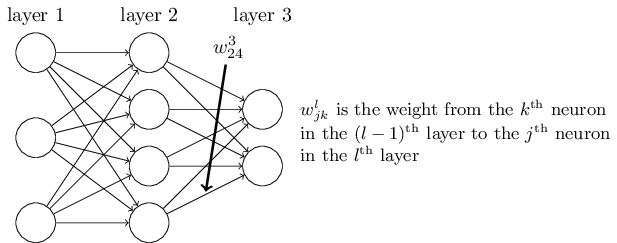
\includegraphics[width=1\linewidth]{fig/02_tikz16} 

}

\caption{Neural Network Notation - w.}\label{fig:bkpg-mv-notation-w}
\end{figure}\begin{figure}

{\centering 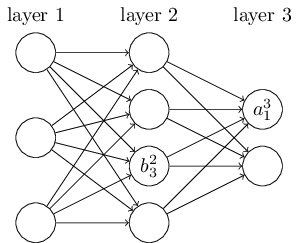
\includegraphics[width=0.5\linewidth]{fig/02_tikz17} 

}

\caption{Neural Network Notation - b.}\label{fig:bkpg-mv-notation-b}
\end{figure}

Then, the activation \(a^l_j\) of the \(j\)th neuron in the \(l\)th
layer is related to the activations in the \((l-1)\)th layer by the
equation

\begin{equation}
a^{l}_j = \sigma\left( \sum_k w^{l}_{jk} a^{l-1}_k + b^l_j \right), \label{eq:bkpg-nvac}
\end{equation}

where the sum is over all neurons \(k\) in the \((l-1)\)th layer.

\subsection{Matrix view of activation
cascading}\label{matrix-view-of-activation-cascading}

To express Equation \eqref{eq:bkpg-nvac} in a matrix form, let \(w^l\)
denote a weight matrix for layer \(l\), the entries of the weight matrix
\(w^l\) are just the weights connecting to the \(l\)th layer of neurons,
that is, the entry in the \(j\)th row and \(k\)th column is
\(w^l_{jk}\). Similarly, let \(b^l\) denote the bias vector for layer
\(l\), the components of the bias vector are just the values \(b^l_j\),
one component for each neuron in the \(l\)th layer. And finally, let
\(a^l\) denote the activation vector for layer \(l\), whose components
are the activations \(a^l_j\). At last, let \(\sigma(v)\) to denote an
elementwise application of a function, such that
\(\sigma(v)_j = \sigma(v_j)\).

Then Equation \eqref{eq:bkpg-nvac} can be rewritten in vectorized form:

\begin{equation} 
a^{l} = \sigma(w^l a^{l-1}+b^l). \label{eq:bkpg-mvac}
\end{equation}

Let us also denote \textbf{\(z^l \equiv w^l a^{l-1}+b^l\)} as the
\textbf{weighted input} to the neurons in layer \(l\) - \(z^l\) has
components \(z^l_j= \sum_k w^l_{jk} a^{l-1}_k+b^l_j\) and \(z^l_j\) in
turns is just the weighted input to the activation function for neuron
\(j\) in layer \(l\). And, it follows that Equation \eqref{eq:bkpg-mvac}
can be rewritten as:

\begin{equation} 
a^{l} = \sigma(z^l), \quad\mbox{and}\quad z^l \equiv w^l a^{l-1}+b^l \label{eq:bkpg-mvaz}
\end{equation}

\section{Two assumptions on cost function for applying
backpropagation}\label{two-assumptions-on-cost-function-for-applying-backpropagation}

\begin{itemize}
\item
  The cost can be written as an average over the cost of individual
  training sample.
\item
  The cost can be written as a function of outputs from the neuron
  network.
\end{itemize}

Thus,

\begin{equation}
C = \frac{1}{n}C_x = \frac{1}{n}\sum_x f_x(a^L, y)
\end{equation}

Why must overall cost as an average of individual training sample costs?
The reason is that backpropagation actually compute the partial
derivatives \(\partial C_x / \partial w\) and
\(\partial C_x / \partial b\) for a single training example, and then
recover \(\partial C / \partial w\) and \(\partial C / \partial b\) by
averaging over training examples.

\section{The Hadamard product (The Schur
product)}\label{the-hadamard-product-the-schur-product}

Let \(s \odot t\) denote the elementwise product of the two vectors:

\begin{equation}
(s \odot t)_j = s_j t_j
\end{equation}

\section{The four fundamental equations behind
backpropagation}\label{the-four-fundamental-equations-behind-backpropagation}

\subsection{Motivation}\label{motivation}

\begin{figure}

{\centering 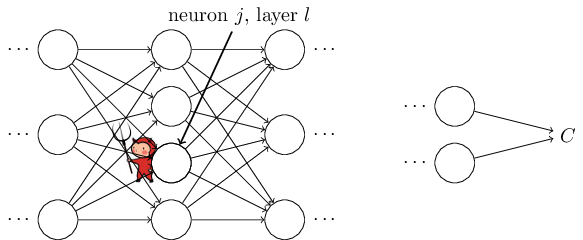
\includegraphics[width=1\linewidth]{fig/02_tikz19} 

}

\caption{Backpropagation - Motivation.}\label{fig:bkpg-demon}
\end{figure}

Imagine a demon sits in neural network at the \(j\)th neuron in \(l\)th
layer. The neuron can change the neuron's weighted input \(z^l_j\) by a
small amount \(\Delta z^l_j\). This change propagates through later
layers in the network, finally causing the overall cost to change by an
amount \(\frac{\partial C}{\partial z^l_j} \Delta z^l_j\). The demon can
lower the overall cost by choosing \(\Delta z^l_j\) to have opposite
sign to \(\frac{\partial C}{\partial z^l_j}\). However, since the demon
is limited to choose a small amount \(\Delta z^l_j\), the cost can be
lower quite a lot when \(\frac{\partial C}{\partial z^l_j}\) is larger,
but not so much when \(\frac{\partial C}{\partial z^l_j}\) is small.
Thus, \(\frac{\partial C}{\partial z^l_j}\) determines how optimal the
neuron \(z^l_j\). And a heuristic sense is that
\(\frac{\partial C}{\partial z^l_j}\) measures the error in the neuron
\(z^l_j\).

Let \(\delta^l_j\) denote the error of neuro \(j\) in layer \(l\):

\begin{equation}
\delta^l_j \equiv \frac{\partial C}{\partial z^l_j}
\end{equation}

\subsection{The equations of
backpropagation}\label{the-equations-of-backpropagation}

The equations are:

\begin{equation}
\begin{array}{cccl}
\mbox{BP1} \quad & \delta^L & = & \nabla_a C \odot \sigma'(z^L) \\
\mbox{BP2} \quad & \delta^l & = & ((w^{l+1})^T \delta^{l+1}) \odot \sigma'(z^l) \\
\mbox{BP3} \quad & \displaystyle \frac{\partial C}{\partial b^l_j} & = & \delta^l_j \\
\mbox{BP4} \quad & \displaystyle \frac{\partial C}{\partial w^l_{jk}} & = & a^{l-1}_k \delta^l_j \\
\end{array}
\end{equation}

The equations are:

\begin{enumerate}
\def\labelenumi{\arabic{enumi}.}
\item
  An equation for the error in the output layer \(\delta^L\).
\item
  An equation for the error \(\delta^l\) in terms of the error in the
  next layer \(\delta^{l+1}\)
\item
  An equation for the rate of change of the cost with respect to any
  bias in the network.
\item
  An equation for the rate of change of the cost with respect to any
  weight in the network.
\end{enumerate}

The equations from a matrix view:

\begin{equation}
\begin{array}{cccl}
\mbox{BP1M} \quad & \delta^L & = & \nabla_a C \odot \sigma'(z^L) \\
                  &          & = & \Sigma'(z^L) \nabla_a C \\
\mbox{BP2M} \quad & \delta^l & = & ((w^{l+1})^T \delta^{l+1}) \odot \sigma'(z^l) \\
                  &          & = & \Sigma'(z^l) (w^{l+1})^T \delta^{l+1} \\
                  &          & = & \Sigma'(z^l) (w^{l+1})^T \ldots \Sigma'(z^{L-1}) (w^L)^T \Sigma'(z^L) \nabla_a C \\
\mbox{BP3M} \quad & \displaystyle \frac{\partial C}{\partial b^l} & = & \delta^l \\
\mbox{BP4M} \quad & \displaystyle \frac{\partial C}{\partial w^l} & = & \delta^l \cdot {a^{l-1}}^T\\
\end{array}
\end{equation}

where \(\Sigma'(z^L)\) is a square matrix whose diagonal entries are the
values \(\sigma'(z^L)\) and whose off-diagonal entries are zero.

A note on Equation BP4:

\begin{equation}  
\frac{\partial C}{\partial w} = a_{\rm in} \delta_{\rm out},
\end{equation}

where it's understood that \(a_{\rm in}\) is the activation of the
neuron input to the weight \(w\), and \(\delta_{\rm out}\) is the error
of the neuron output from the weight \(w\).

\begin{figure}

{\centering 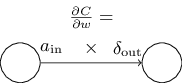
\includegraphics[width=0.5\linewidth]{fig/02_tikz20} 

}

\caption{Backpropagation - BP4.}\label{fig:bkpg-eq4}
\end{figure}

when the activation \(a_{\rm in}\) is small, \(a_{\rm in} \approx 0\),
the gradient term \(\partial C / \partial w\) will also tend to be
small, and as a result, weight learns slowly, meaning that it's not
changing much during gradient descent. \textbf{Thus, weights will learn
slowly if input neuron is low-activation.}

A note on Equation BP1:

\begin{figure}

{\centering 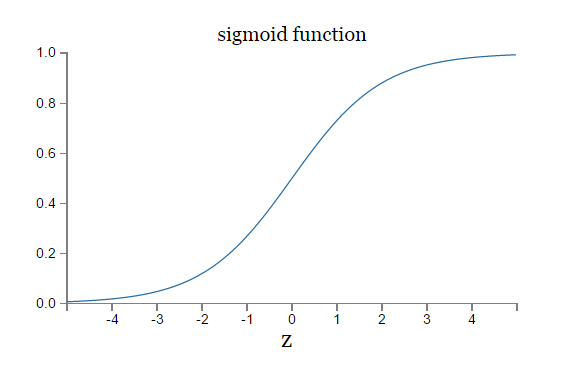
\includegraphics[width=0.5\linewidth]{fig/02_sigmoid} 

}

\caption{Backpropagation - BP1.}\label{fig:bkpg-eq1}
\end{figure}

when \(\sigma(z^L_j) \to 0 \mbox{or} 1\), \(\sigma'(z^L_j) \approx 0\),
the gradient \(\partial C / \partial w \approx 0\), and the weight
learns slowly. \textbf{Thus, weights will learn slowly if output neuron
is either low-activation or high activation.}

These insight provide a guidance on designing activation functions which
have particular desired learning properties, e.g., a (non-sigmoid)
activation function \(\sigma(\cdot)\) that has \(\sigma'(\cdot)\) stays
positive and never gets close to zero could prevent the learning rate
slow-down which occurs when ordinary sigmoid neurons saturate.

\section{The proof of backpropagation
equations:}\label{the-proof-of-backpropagation-equations}

\begin{itemize}
\tightlist
\item
  BP1:
\end{itemize}

\begin{equation}  
\delta^L_j = \frac{\partial C}{\partial z^L_j} 
           = \sum_k \frac{\partial C}{\partial a^L_k} \frac{\partial a^L_k}{\partial z^L_j}
           = \frac{\partial C}{\partial a^L_j} \frac{\partial a^L_j}{\partial z^L_j} 
           = \frac{\partial C}{\partial a^L_j} \sigma'(z^L_j).
\end{equation}

\begin{itemize}
\tightlist
\item
  BP2:
\end{itemize}

\begin{equation}  
\delta^l_j = \frac{\partial C}{\partial z^l_j}
           = \sum_k \frac{\partial C}{\partial z^{l+1}_k} \frac{\partial z^{l+1}_k}{\partial z^l_j} 
           = \sum_k \frac{\partial z^{l+1}_k}{\partial z^l_j} \delta^{l+1}_k
\end{equation}

plugin:

\begin{equation}
z^{l+1}_k = \sum_j w^{l+1}_{kj} a^l_j +b^{l+1}_k = \sum_j w^{l+1}_{kj} \sigma(z^l_j) +b^{l+1}_k 
\quad \implies \quad 
\frac{\partial z^{l+1}_k}{\partial z^l_j} = w^{l+1}_{kj} \sigma'(z^l_j)
\end{equation}

give:

\begin{equation}
\delta^l_j = \sum_k w^{l+1}_{kj}  \delta^{l+1}_k \sigma'(z^l_j).
\end{equation}

\begin{itemize}
\tightlist
\item
  BP3:
\end{itemize}

\begin{equation}
\displaystyle \frac{\partial C}{\partial b^l_j} 
  = \sum_k \frac{\partial C}{\partial z^l_k} \frac{\partial z^l_k}{\partial b^l_j}
  = \frac{\partial C}{\partial z^l_j} \frac{\partial z^l_j}{\partial b^l_j}
  = \delta^l_j.
\end{equation}

\begin{itemize}
\tightlist
\item
  BP4:
\end{itemize}

\begin{equation}
\displaystyle \frac{\partial C}{\partial w^l_{jk}} 
  = \sum_i \frac{\partial C}{\partial z^l_i} \frac{\partial z^l_i}{\partial w^l_{jk}}
  = \frac{\partial C}{\partial z^l_j} \frac{\partial z^l_j}{\partial w^l_{jk}}
  = a^{l-1}_k \delta^l_j.
\end{equation}

\section{The backpropagation
algorithm}\label{the-backpropagation-algorithm}

The backpropagation equations provide a way of computing the gradient of
the cost function:

\begin{enumerate}
\def\labelenumi{\arabic{enumi}.}
\item
  Input \(x\): Set the corresponding activation \(a^1\) for the input
  layer.
\item
  Feedforward: For each layer \(l = 2, 3, \ldots, L\), compute
  \(z^l = w^l a^{l-1} + b^l\) and \(a^l = \sigma(z^l)\).
\item
  Output error \(\delta^L\): Compute the vector
  \(\delta^L = \nabla_a C \odot \sigma'(z^L) = \Sigma'(z^L) \nabla_a C\).
\item
  Backpropagate the error: For each \(l = L -1, L - 2, \ldots, 2\),
  compute
  \(\delta^l = ((w^{l+1})^T \delta^{l+1}) \odot \sigma'(z^l) = \Sigma'(z^l) (w^{l+1})^T \delta^{l+1}\).
\item
  Output: The gradient of the cost function is given by
  \(\displaystyle \frac{\partial C}{\partial w^l_{jk}} = a^{l-1}_k \delta^l_j\)
  and \(\displaystyle \frac{\partial C}{\partial b^l_j} = \delta^l_j\).
\end{enumerate}

In context of a learning algorithm, such as stochastic gradient descent,
often computes the gradient for many training examples, e.g., a
mini-batch of \(m\) training example and applies a gradient descent
learning step based on that mini-batch:

\begin{enumerate}
\def\labelenumi{\arabic{enumi}.}
\item
  Input a set of \(m\) training examples.
\item
  For each training example \(x\): Set the corresponding input
  activation \(a^{x, 1}\) and perform the backpropagtion algorithm:

  \begin{itemize}
  \item
    Feedforward: For each layer \(l = 2, 3, \ldots, L\), compute
    \(z^{x, l} = w^l a^{x, l-1} + b^l\) and
    \(a^{x, l} = \sigma(z^{x, l})\).
  \item
    Output error \(\delta^{x, L}\): Compute the vector
    \(\delta^{x, L} = \nabla_a C \odot \sigma'(z^{x, L}) = \Sigma'(z^{x, L}) \nabla_a C\).
  \item
    Backpropagate the error: For each \(l = L -1, L - 2, \ldots, 2\),
    compute
    \(\delta^{x, l} = ((w^{l+1})^T \delta^{x, l+1}) \odot \sigma'(z^{x, l}) = \Sigma'(z^{x, l}) (w^{l+1})^T \delta^{x, l+1}\).
  \end{itemize}
\item
  Gradient descent: For each \(l = L, L - 1, \ldots, 2\) update the
  weights and bias according the rule:
  \[w^l \rightarrow w^l-\frac{\eta}{m} \sum_x \delta^{x,l} (a^{x,l-1})^T  \quad\mbox{and}\quad b^l \rightarrow b^l-\frac{\eta}{m} \sum_x \delta^{x,l}\].
\end{enumerate}

In practice, implement stochastic gradient descent would require an
outer loop generating mini-batches of training examples, and an outer
loop stepping through multiple epochs of training.

\section{The code for
backpropagation}\label{the-code-for-backpropagation}

See code and note on \texttt{network.py} and \texttt{network\_matrix.py}
in \href{./src}{source code folder}.

\section{The big picture}\label{the-big-picture}

\begin{figure}

{\centering 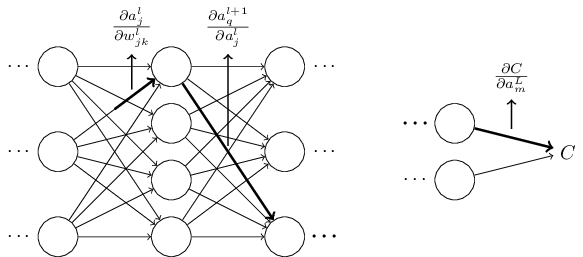
\includegraphics[width=1\linewidth]{fig/02_tikz27} 

}

\caption{Backpropagation - Intuition}\label{fig:bkpg-init}
\end{figure}

\begin{equation} 
\Delta C \approx \frac{\partial C}{\partial w^l_{jk}} \Delta w^l_{jk}
         \approx \sum_{mnp\ldots q} 
                 \frac{\partial C}{\partial a^L_m} 
                 \frac{\partial a^L_m}{\partial a^{L-1}_n}
                 \frac{\partial a^{L-1}_n}{\partial a^{L-2}_p} \ldots
                 \frac{\partial a^{l+1}_q}{\partial a^l_j} 
                 \frac{\partial a^l_j}{\partial w^l_{jk}} \Delta w^l_{jk},
\end{equation}

As a result,

\begin{equation} 
\frac{\partial C}{\partial w^l_{jk}} = \sum_{mnp\ldots q} 
  \frac{\partial C}{\partial a^L_m} 
  \frac{\partial a^L_m}{\partial a^{L-1}_n}
  \frac{\partial a^{L-1}_n}{\partial a^{L-2}_p} \ldots
  \frac{\partial a^{l+1}_q}{\partial a^l_j} 
  \frac{\partial a^l_j}{\partial w^l_{jk}}
\end{equation}

Backpropgation can be viewed as a way of calculating all sum
\(mnp \ldots q\) stepwise by absorbing previous computation - stepwise
of hyper matrix multiplication.

\chapter{Improving the way neural networks learn}\label{ipln}

\section{The cross-entropy cost
function}\label{the-cross-entropy-cost-function}

In information theory, the cross entropy between two probability
distributions \({\displaystyle p}\) and \({\displaystyle q}\) over the
same underlying set of events measures the average number of
\textbf{bits} needed to identify an event drawn from the set, if a
coding scheme is used that is optimized for an ``unnatural''"
probability distribution \({\displaystyle q}\), rather than the ``true''
distribution \({\displaystyle p}\).

The cross entropy for the distributions \({\displaystyle p}\) and
\({\displaystyle q}\) over a given set is defined as follows:

\begin{equation}
\displaystyle H(p,q) = \operatorname{E}_{p}[-\log q] = H(p) + D_{\mathrm{KL}}(p\|q),
\end{equation}

where \({\displaystyle H(p)}\) is the entropy of \({\displaystyle p}\),
and \({\displaystyle D_{\mathrm {KL}}(p||q)}\) is the Kullback-Leibler
divergence of \({\displaystyle q}\) from \({\displaystyle p}\) (also
known as the relative entropy of p with respect to q - note the reversal
of emphasis).

For discrete \({\displaystyle p}\) and \({\displaystyle q}\) this means

\begin{equation}
\displaystyle H(p,q) = - \sum_{x} p(x) \log q(x)
\end{equation}

The situation for continuous distributions is analogous:

\begin{equation}
\displaystyle H(p,q) = -\int_{X} p(x) \log q(x) dx.
\end{equation}

NB: The notation \({\displaystyle H(p,q)}\) is also used for a different
concept, the joint entropy of \({\displaystyle p}\) and
\({\displaystyle q}\).

\subsection{Connect output layer activation function with cost
function}\label{connect-output-layer-activation-function-with-cost-function}

From Backpropgation
\(\mbox{BP1}\quad\delta^L = \nabla_a C \odot f'(z^L)\):

\begin{enumerate}
\def\labelenumi{\arabic{enumi}.}
\item
  If sigmoid activation function
  \(a = f(z) = \sigma(z) = \displaystyle \frac{1}{1+e^{-z}}\), and
  cross-entropy cost function
  \(C = -\sum_{j}\left[y_j\ln(a_j^L)+(1-y_j)\ln(1-a_j^L)\right]\), then
  \(\delta^L = a^L-y\).
\item
  If linear activation function \(a = f(z) = z\), and quadratic cost
  function \(C = \sum_j\left(y_j - a_j^L\right)^2\), then
  \(\delta^L = a^L-y\).
\item
  If softmax activation function
  \(a_j^L = \frac{e^{z_j^L}}{\sum_k e^{z_k^L}}\), and log-likelihood
  cost function \(C = -\ln(y^Ta^L)\), then \(\delta^L = a^L-y\).
\end{enumerate}

Here, \(C\) is the cost function of \(a^L\) and \(f\) is the output
layer activation function.

TODO: add more from book

It tells us that the rate at which the weight learns is controlled by
\(\sigma(z) - y\), i.e., by the error in the output. The larger the
error, the faster the neuron will learn.

In fact, the cross-entropy is nearly always the better choice, provided
the output neurons are sigmoid neurons.

Using the quadratic cost when we have linear neurons in the output layer

In Chapter 1 we used the quadratic cost and a learning rate of
η=3.0η=3.0. As discussed above, it's not possible to say precisely what
it means to use the ``same'' learning rate when the cost function is
changed. For both cost functions I experimented to find a learning rate
that provides near-optimal performance, given the other hyper-parameter
choices.

There is, incidentally, a very rough general heuristic for relating the
learning rate for the cross-entropy and the quadratic cost. As we saw
earlier, the gradient terms for the quadratic cost have an extra
σ′=σ(1−σ)σ′=σ(1−σ) term in them. Suppose we average this over values for
σσ, ∫10dσσ(1−σ)=1/6∫01dσσ(1−σ)=1/6. We see that (very roughly) the
quadratic cost learns an average of 66 times slower, for the same
learning rate. This suggests that a reasonable starting point is to
divide the learning rate for the quadratic cost by 66. Of course, this
argument is far from rigorous, and shouldn't be taken too seriously.
Still, it can sometimes be a useful starting point.

\section{What does the cross-entropy mean? Where does it come from?
Origination of cross-entropy
cost}\label{what-does-the-cross-entropy-mean-where-does-it-come-from-origination-of-cross-entropy-cost}

\subsection{\texorpdfstring{what could have \textbf{motivated} us to
think up the cross-entropy in the first
place?}{what could have motivated us to think up the cross-entropy in the first place?}}\label{what-could-have-motivated-us-to-think-up-the-cross-entropy-in-the-first-place}

deriviation

\subsection{What about the intuitive meaning of the
cross-entropy?}\label{what-about-the-intuitive-meaning-of-the-cross-entropy}

\section{Softmax}\label{softmax}

Given this similarity, should you use a sigmoid output layer and
cross-entropy, or a softmax output layer and log-likelihood?

As a more general point of principle, softmax plus log-likelihood is
worth using whenever you want to interpret the output activations as
probabilities. That's not always a concern, but can be useful with
classification problems (like MNIST) involving disjoint classes.

Where does the ``softmax'' name come from?

\begin{equation}
a^L_j = \frac{e^{c z^L_j}}{\sum_k e^{c z^L_k}},
\end{equation}

if \(c \rightarrow \infty\) then
\(a^L_j = 1 if z^L_j = max{z^L_k, k = 1, \ldots, m} and 0 otherwise\),
so the \(c = 1\) function as a ``softened'' version of the maximum
function. This is the origin of the term ``softmax''.

\subsection{Backpropagation with softmax and the log-likelihood
cost}\label{backpropagation-with-softmax-and-the-log-likelihood-cost}

derive the expression

\begin{equation}
\delta^L_j \equiv \partial C / \partial z^L_j = \ldots = a^L_j -y_j
\end{equation}

fill in \(ldots\)

\section{Overfitting and
regularization}\label{overfitting-and-regularization}

John von Neumann famously said

With four parameters I can fit an elephant, and with five I can make him
wiggle his trunk.

\url{http://www.johndcook.com/blog/2011/06/21/how-to-fit-an-elephant/}

\begin{Shaded}
\begin{Highlighting}[]
\CommentTok{"""}
\CommentTok{Author: Piotr A. Zolnierczuk (zolnierczukp at ornl dot gov)}
\CommentTok{ }
\CommentTok{Based on a paper by:}
\CommentTok{Drawing an elephant with four complex parameters}
\CommentTok{Jurgen Mayer, Khaled Khairy, and Jonathon Howard,}
\CommentTok{Am. J. Phys. 78, 648 (2010), DOI:10.1119/1.3254017}
\CommentTok{"""}
\ImportTok{import} \NormalTok{numpy }\ImportTok{as} \NormalTok{np}
\ImportTok{import} \NormalTok{pylab}
 
\CommentTok{# elephant parameters}
\NormalTok{p1, p2, p3, p4 }\OperatorTok{=} \NormalTok{(}\DecValTok{50} \OperatorTok{-} \NormalTok{30j, }\DecValTok{18} \OperatorTok{+}  \NormalTok{8j, }\DecValTok{12} \OperatorTok{-} \NormalTok{10j, }\OperatorTok{-}\DecValTok{14} \OperatorTok{-} \NormalTok{60j )}
\NormalTok{p5 }\OperatorTok{=} \DecValTok{40} \OperatorTok{+}\OtherTok{ 20j} \CommentTok{# eyepiece}
 
\KeywordTok{def} \NormalTok{fourier(t, C):}
    \NormalTok{f }\OperatorTok{=} \NormalTok{np.zeros(t.shape)}
    \NormalTok{A, B }\OperatorTok{=} \NormalTok{C.real, C.imag}
    \ControlFlowTok{for} \NormalTok{k }\OperatorTok{in} \BuiltInTok{range}\NormalTok{(}\BuiltInTok{len}\NormalTok{(C)):}
        \NormalTok{f }\OperatorTok{=} \NormalTok{f }\OperatorTok{+} \NormalTok{A[k]}\OperatorTok{*}\NormalTok{np.cos(k}\OperatorTok{*}\NormalTok{t) }\OperatorTok{+} \NormalTok{B[k]}\OperatorTok{*}\NormalTok{np.sin(k}\OperatorTok{*}\NormalTok{t)}
    \ControlFlowTok{return} \NormalTok{f}
 
\KeywordTok{def} \NormalTok{elephant(t, p1, p2, p3, p4, p5):}
    \NormalTok{npar }\OperatorTok{=} \DecValTok{6}
    \NormalTok{Cx }\OperatorTok{=} \NormalTok{np.zeros((npar,), dtype}\OperatorTok{=}\StringTok{'complex'}\NormalTok{)}
    \NormalTok{Cy }\OperatorTok{=} \NormalTok{np.zeros((npar,), dtype}\OperatorTok{=}\StringTok{'complex'}\NormalTok{)}
 
    \NormalTok{Cx[}\DecValTok{1}\NormalTok{] }\OperatorTok{=} \NormalTok{p1.real}\OperatorTok{*}\NormalTok{1j}
    \NormalTok{Cx[}\DecValTok{2}\NormalTok{] }\OperatorTok{=} \NormalTok{p2.real}\OperatorTok{*}\NormalTok{1j}
    \NormalTok{Cx[}\DecValTok{3}\NormalTok{] }\OperatorTok{=} \NormalTok{p3.real}
    \NormalTok{Cx[}\DecValTok{5}\NormalTok{] }\OperatorTok{=} \NormalTok{p4.real}
 
    \NormalTok{Cy[}\DecValTok{1}\NormalTok{] }\OperatorTok{=} \NormalTok{p4.imag }\OperatorTok{+} \NormalTok{p1.imag}\OperatorTok{*}\NormalTok{1j}
    \NormalTok{Cy[}\DecValTok{2}\NormalTok{] }\OperatorTok{=} \NormalTok{p2.imag}\OperatorTok{*}\NormalTok{1j}
    \NormalTok{Cy[}\DecValTok{3}\NormalTok{] }\OperatorTok{=} \NormalTok{p3.imag}\OperatorTok{*}\NormalTok{1j}
 
    \NormalTok{x }\OperatorTok{=} \NormalTok{np.append(fourier(t,Cx), [}\OperatorTok{-}\NormalTok{p5.imag])}
    \NormalTok{y }\OperatorTok{=} \NormalTok{np.append(fourier(t,Cy), [p5.imag])}
 
    \ControlFlowTok{return} \NormalTok{x,y}
 
\NormalTok{x, y }\OperatorTok{=} \NormalTok{elephant(np.linspace(}\DecValTok{0}\NormalTok{,}\DecValTok{2}\OperatorTok{*}\NormalTok{np.pi,}\DecValTok{1000}\NormalTok{), p1, p2, p3, p4, p5)}
\NormalTok{pylab.plot(y,}\OperatorTok{-}\NormalTok{x,}\StringTok{'.'}\NormalTok{)}
\NormalTok{pylab.show()}
\end{Highlighting}
\end{Shaded}

\subsection{Regularization}\label{regularization}

These are known as regularization techniques. In this section I describe
one of the most commonly used regularization techniques, a technique
sometimes known as weight decay or L2 regularization. The idea of L2
regularization is to add an extra term to the cost function, a term
called the regularization term. Here's the regularized cross-entropy:

\begin{eqnarray}
C = -\frac{1}{n} \sum_{xj} \left[ y_j \ln a^L_j+(1-y_j) \ln (1-a^L_j)\right] + \frac{\lambda}{2n} \sum_w w^2.
\tag{85}\end{eqnarray}

This is scaled by a factor λ/2nλ/2n, where
λ\textgreater{}0λ\textgreater{}0 is known as the regularization
parameter, and nn is, as usual, the size of our training set.

\begin{eqnarray} C = \frac{1}{2n} \sum_x \|y-a^L\|^2 +
  \frac{\lambda}{2n} \sum_w w^2.
\tag{86}\end{eqnarray}

\begin{eqnarray}  C = C_0 + \frac{\lambda}{2n}
\sum_w w^2,
\tag{87}\end{eqnarray}

where C0C0 is the original, unregularized cost function.

Intuitively, the effect of regularization is to make it so the network
prefers to learn small weights, all other things being equal. Large
weights will only be allowed if they considerably improve the first part
of the cost function. Put another way, regularization can be viewed as a
way of compromising between finding small weights and minimizing the
original cost function. The relative importance of the two elements of
the compromise depends on the value of λλ: when λλ is small we prefer to
minimize the original cost function, but when λλ is large we prefer
small weights.

\subsubsection{why regularization
works?}\label{why-regularization-works}

Suppose our network mostly has small weights, as will tend to happen in
a regularized network. The smallness of the weights means that the
behaviour of the network won't change too much if we change a few random
inputs here and there. That makes it difficult for a regularized network
to learn the effects of local noise in the data. Think of it as a way of
making it so single pieces of evidence don't matter too much to the
output of the network. Instead, a regularized network learns to respond
to types of evidence which are seen often across the training set. By
contrast, a network with large weights may change its behaviour quite a
bit in response to small changes in the input.

It has been conjectured that ``the dynamics of gradient descent learning
in multilayer nets has a `self-regularization' effect'' - In
Gradient-Based Learning Applied to Document Recognition, by Yann LeCun,
Léon Bottou, Yoshua Bengio, and Patrick Haffner (1998).

it's worth noting that having a large bias doesn't make a neuron
sensitive to its inputs in the same way as having large weights

\subsubsection{Other techniques for
regularization}\label{other-techniques-for-regularization}

Three other approaches to reducing overfitting: L1 regularization,
dropout, and artificially increasing the training set size.

L1 regularization: In this approach we modify the unregularized cost
function by adding the sum of the absolute values of the weights:

\begin{eqnarray}
C = C_0 + \frac{\lambda}{n} \sum_w |w|.
\tag{95}\end{eqnarray}

The partial derivatives of the cost function

\begin{eqnarray}  
\frac{\partial C}{\partial w} = \frac{\partial C_0}{\partial w} + \frac{\lambda}{n} \, {\rm sgn}(w),
\tag{96}\end{eqnarray}

where \(sgn(w)\) is the sign of ww, that is, \(+1\) if \(w\) is
positive, and \(-1\) if \(w\) is negative.

The resulting update rule for an L1 regularized network is:

\begin{eqnarray}  
w \rightarrow w' = w - \frac{\eta \lambda}{n} \mbox{sgn}(w) - \eta \frac{\partial C_0}{\partial w},
\tag{97}\end{eqnarray}

where, as per usual, we can estimate \(∂C0/∂w\) using a mini-batch
average, if we wish.

The net result is that L1 regularization tends to concentrate the weight
of the network in a relatively small number of high-importance
connections, while the other weights are driven toward zero.

NB: \(∂C/∂w\) isn't defined when \(w=0\), use with the convention that
\(sgn(0)=0\).

\paragraph{dropout}\label{dropout}

Ordinarily, we'd train by forward-propagating xx through the network,
and then backpropagating to determine the contribution to the gradient.
With dropout, this process is modified. We start by randomly (and
temporarily) deleting half the hidden neurons in the network, while
leaving the input and output neurons untouched. After doing this, we'll
end up with a network along the following lines. Note that the dropout
neurons, i.e., the neurons which have been temporarily deleted, are
still ghosted in:

This kind of averaging scheme is often found to be a powerful (though
expensive) way of reducing overfitting. The reason is that the different
networks may overfit in different ways, and averaging may help eliminate
that kind of overfitting. \ldots{} Think dropout as a less cost version
of model averaging - voting.

What's this got to do with dropout? Heuristically, when we dropout
different sets of neurons, it's rather like we're training different
neural networks. And so the dropout procedure is like averaging the
effects of a very large number of different networks. The different
networks will overfit in different ways, and so, hopefully, the net
effect of dropout will be to reduce overfitting.

``This technique reduces complex co-adaptations of neurons, since a
neuron cannot rely on the presence of particular other neurons. It is,
therefore, forced to learn more robust features that are useful in
conjunction with many different random subsets of the other neurons.'' -
ImageNet Classification with Deep Convolutional Neural Networks, by Alex
Krizhevsky, Ilya Sutskever, and Geoffrey Hinton (2012).

In other words, if we think of our network as a model which is making
predictions, then we can think of dropout as a way of making sure that
the model is robust to the loss of any individual piece of evidence. In
this, it's somewhat similar to L1 and L2 regularization, which tend to
reduce weights, and thus make the network more robust to losing any
individual connection in the network.

The original paper introducing the dropout technique: Improving neural
networks by preventing co-adaptation of feature detectors by Geoffrey
Hinton, Nitish Srivastava, Alex Krizhevsky, Ilya Sutskever, and Ruslan
Salakhutdinov (2012). Dropout has been especially useful in training
large, deep networks, where the problem of overfitting is often acute.

\subsubsection{Artificially expanding the training
data}\label{artificially-expanding-the-training-data}

Best Practices for Convolutional Neural Networks Applied to Visual
Document Analysis, by Patrice Simard, Dave Steinkraus, and John Platt
(2003).: then they expanded the training data, using not just rotations,
as I described above, but also translating and skewing the images. By
training on the expanded data set they increased their network's
accuracy to 98.9 percent. They also experimented with what they called
``elastic distortions'', a special type of image distortion intended to
emulate the random oscillations found in hand muscles. By using the
elastic distortions to expand the data they achieved an even higher
accuracy, 99.3 percent. Effectively, they were broadening the experience
of their network by exposing it to the sort of variations that are found
in real handwriting.

\subsection{weight initialization}\label{weight-initialization}

examples of neural networks where the long-run behaviour is
significantly better with the \(1/\sqrt{n_{\mathrm in}}\) weight
initialization. Thus it's not only the speed of learning which is
improved, it's sometimes also the final performance.

Practical Recommendations for Gradient-Based Training of Deep
Architectures, by Yoshua Bengio (2012).

provided \(\eta \lambda \ll n\) the weights will decay by a factor of
\(exp(−\eta\lambda/m)\) per epoch:

\begin{equation}
decay (1 - \eta\lambda / n)^{n / m} per epoche, as n \rightarrow \infty , it goes to exp(-\eta\lambda/n\times n /m)
\end{equation}

\section{the code}\label{the-code}

Modify the code above to implement L1 regularization, and use L1
regularization to classify MNIST digits using a 3030 hidden neuron
network.

\section{How to choose a neural network's
hyper-parameters?}\label{how-to-choose-a-neural-networks-hyper-parameters}

broad strategy: And so I'd like to re-emphasize that during the early
stages you should make sure you can get quick feedback from experiments.

learning rate: An even better approach would be to start with
\(\eta = 0.25\), train for 2020 epochs, and then switch to
\(\eta = 0.025\).

You may optionally refine your estimate, to pick out the largest value
of \(\eta\) at which the cost decreases during the first few epochs

In fact, we'll use validation accuracy to pick the regularization
hyper-parameter, the mini-batch size, and network parameters such as the
number of layers and hidden neurons, and so on. Why do things
differently for the learning rate? Frankly, this choice is my personal
aesthetic preference, and is perhaps somewhat idiosyncratic. The
reasoning is that the other hyper-parameters are intended to improve the
final classification accuracy on the test set, and so it makes sense to
select them on the basis of validation accuracy. However, the learning
rate is only incidentally meant to impact the final classification
accuracy. Its primary purpose is really to control the step size in
gradient descent, and monitoring the training cost is the best way to
detect if the step size is too big. With that said, this is a personal
aesthetic preference.

Use early stopping to determine the number of training epochs:
no-improvement-in-ten rule

Learning rate schedule: How should we set our learning rate schedule?
Many approaches are possible. One natural approach is to use the same
basic idea as early stopping. The idea is to hold the learning rate
constant until the validation accuracy starts to get worse. Then
decrease the learning rate by some amount, say a factor of two or ten.
We repeat this many times, until, say, the learning rate is a factor of
1,024 (or 1,000) times lower than the initial value. Then we terminate.

A readable recent paper which demonstrates the benefits of variable
learning rates in attacking MNIST is Deep, Big, Simple Neural Nets Excel
on Handwritten Digit Recognition, by Dan Claudiu Cireșan, Ueli Meier,
Luca Maria Gambardella, and Jürgen Schmidhuber (2010).

The regularization parameter, λλ: I suggest starting initially with no
regularization (λ=0.0λ=0.0), and determining a value for ηη, as above.
Using that choice of ηη, we can then use the validation data to select a
good value for λλ. Start by trialling λ=1.0 and then increase or
decrease by factors of 10, as needed to improve performance on the
validation data. Once you've found a good order of magnitude, you can
fine tune your value of λλ. That done, you should return and re-optimize
ηη again.

Mini-batch size: Fortunately, the choice of mini-batch size at which the
speed is maximized is relatively independent of the other
hyper-parameters (apart from the overall architecture), so you don't
need to have optimized those hyper-parameters in order to find a good
mini-batch size.

The way to go is therefore to use some acceptable (but not necessarily
optimal) values for the other hyper-parameters, and then trial a number
of different mini-batch sizes, scaling ηη as above. Plot the validation
accuracy versus time (as in, real elapsed time, not epoch!), and choose
whichever mini-batch size gives you the most rapid improvement in
performance. With the mini-batch size chosen you can then proceed to
optimize the other hyper-parameters.

Automated techniques: grid search

Random search for hyper-parameter optimization, by James Bergstra and
Yoshua Bengio (2012).

I won't review all that work here, but do want to mention a particularly
promising 2012 paper which used a Bayesian approach to automatically
optimize hyper-parameters - Practical Bayesian optimization of machine
learning algorithms, by Jasper Snoek, Hugo Larochelle, and Ryan Adams.

code at: \url{https://github.com/jaberg/hyperopt}

Sum up:

Efficient BackProp, by Yann LeCun, Léon Bottou, Genevieve Orr and
Klaus-Robert Müller (1998)

Practical recommendations for gradient-based training of deep
architectures, by Yoshua Bengio (2012).

Neural Networks: Tricks of the Trade, edited by Grégoire Montavon,
Geneviève Orr, and Klaus-Robert Müller.

\section{Other techniques}\label{other-techniques}

Hessian

Momentum-based gradient descent: Intuitively, the advantage Hessian
optimization has is that it incorporates not just information about the
gradient, but also information about how the gradient is changing.

What would go wrong if we used \(\mu > 1\) in the momentum technique?
What would go wrong if we used \(\mu < 0\) in the momentum technique?

Add momentum-based stochastic gradient descent to network2.py.

Other approaches to minimizing the cost function:

On the importance of initialization and momentum in deep learning, by
Ilya Sutskever, James Martens, George Dahl, and Geoffrey Hinton (2012).

\section{Other models of artificial
neuron}\label{other-models-of-artificial-neuron}

tanh

Efficient BackProp, by Yann LeCun, Léon Bottou, Genevieve Orr and
Klaus-Robert Müller (1998), and Understanding the difficulty of training
deep feedforward networks, by Xavier Glorot and Yoshua Bengio (2010).

rectified linear

Some recent work on image recognition has found considerable benefit in
using rectified linear units through much of the network.

For example, What is the Best Multi-Stage Architecture for Object
Recognition?, by Kevin Jarrett, Koray Kavukcuoglu, Marc'Aurelio Ranzato
and Yann LeCun (2009), Deep Sparse Rectifier Neural Networks, by Xavier
Glorot, Antoine Bordes, and Yoshua Bengio (2011), and ImageNet
Classification with Deep Convolutional Neural Networks, by Alex
Krizhevsky, Ilya Sutskever, and Geoffrey Hinton (2012). Note that these
papers fill in important details about how to set up the output layer,
cost function, and regularization in networks using rectified linear
units. I've glossed over all these details in this brief account. The
papers also discuss in more detail the benefits and drawbacks of using
rectified linear units. Another informative paper is Rectified Linear
Units Improve Restricted Boltzmann Machines, by Vinod Nair and Geoffrey
Hinton (2010), which demonstrates the benefits of using rectified linear
units in a somewhat different approach to neural networks.

\chapter{A visual proof that neural nets can compute any
function}\label{vsnn}

The universality theorem: \textbf{Neural networks with a single hidden
layer} can be used to \textbf{approximate} any \textbf{continuous
function} to any \textbf{desired precision}.

\section{Universality with one input and one
output}\label{universality-with-one-input-and-one-output}

Let \(w \to \infty\) and \(b = -sw\), then \(\sigma(wx+b)\) approximate
a step function stepping at \(x = s\). Two hidden neurons step up at
\(s_1\) and step down at \(s_2\) resepectively can approximate a bump
function over interval \((s_1, s_2)\). An infinite number of such two
neurons structure together can appromixate an inifinite disected
\(\sigma^{-1} \circ f(x)\). As a result, the output from such single
hidden layer neural network approximate \(f(x)\) to any desired
precision.

\begin{figure}

{\centering 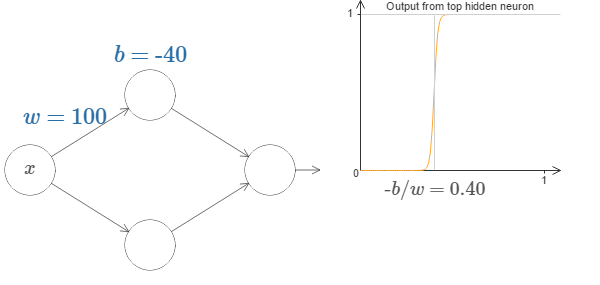
\includegraphics[width=0.75\linewidth]{fig/04_tikz41} 

}

\caption{Neural Network Universality - 1.}\label{fig:vsnn-nnup-01}
\end{figure}

\begin{figure}

{\centering 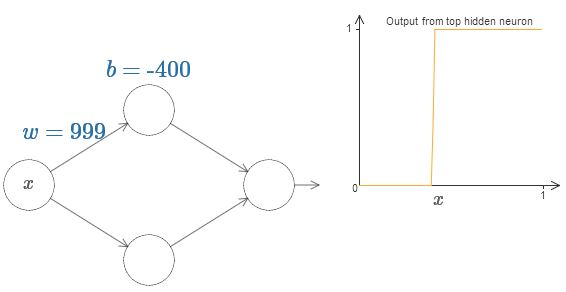
\includegraphics[width=0.75\linewidth]{fig/04_tikz42} 

}

\caption{Neural Network Universality - 2.}\label{fig:vsnn-nnup-02}
\end{figure}

\begin{figure}

{\centering 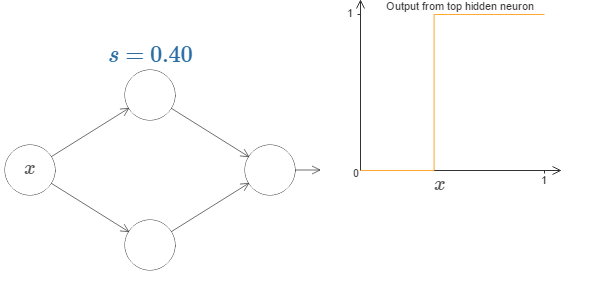
\includegraphics[width=0.75\linewidth]{fig/04_tikz43} 

}

\caption{Neural Network Universality - 3.}\label{fig:vsnn-nnup-03}
\end{figure}

\begin{figure}

{\centering 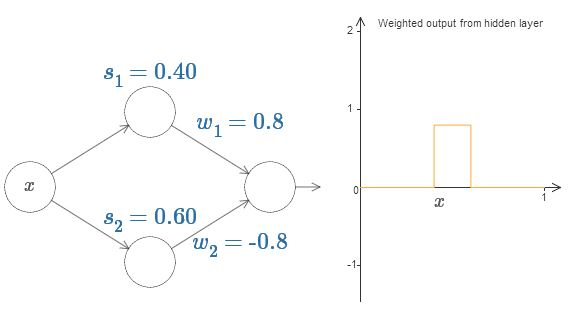
\includegraphics[width=0.75\linewidth]{fig/04_tikz44} 

}

\caption{Neural Network Universality - 4.}\label{fig:vsnn-nnup-04}
\end{figure}

\begin{figure}

{\centering 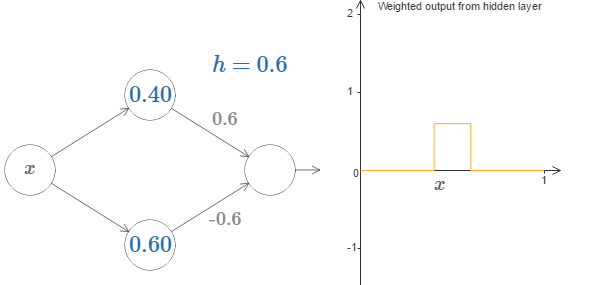
\includegraphics[width=0.75\linewidth]{fig/04_tikz45} 

}

\caption{Neural Network Universality - 5.}\label{fig:vsnn-nnup-05}
\end{figure}

\begin{figure}

{\centering 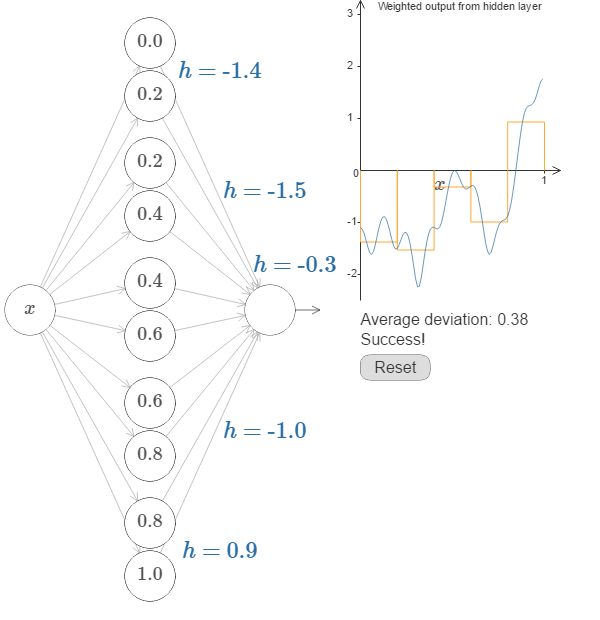
\includegraphics[width=0.75\linewidth]{fig/04_tikz46} 

}

\caption{Neural Network Universality - 6.}\label{fig:vsnn-nnup-06}
\end{figure}

\section{Universality with multiple input and multiple
output}\label{universality-with-multiple-input-and-multiple-output}

The crucial in universality is constructing the step function and then
the bump function on high dimension. A two hidden layer neural network
solution is constructing step function on each dimension and combine
such step functions into bump function.

\begin{figure}

{\centering 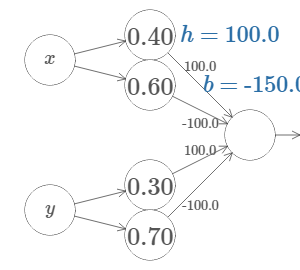
\includegraphics[width=0.5\linewidth]{fig/04_tikz47} 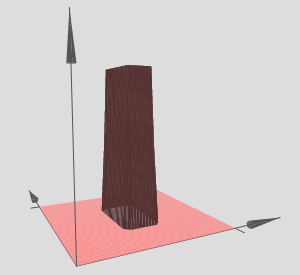
\includegraphics[width=0.5\linewidth]{fig/04_tikz47_2} 

}

\caption{Neural Network Universality - 7.}\label{fig:vsnn-nnup-07}
\end{figure}

\begin{figure}

{\centering 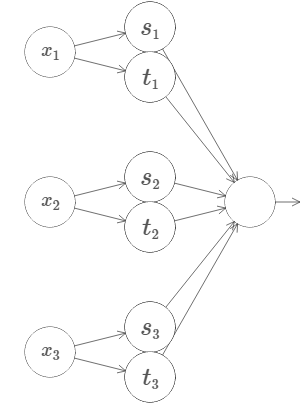
\includegraphics[width=0.4\linewidth]{fig/04_tikz48} 

}

\caption{Neural Network Universality - 8.}\label{fig:vsnn-nnup-08}
\end{figure}

Again, let all weights in the first layer go infinity and bias
proportion to weights such that \(s_1, t_1, s_2, t_2, \ldots\) are the
step points, and the weights in the second layer alternate \(+h, -h\)
where \(h\) is very large, and bias \((-m + 1/2)h\) where \(m\) is the
input dimension. As a result, such neural network can approximate any
multiple input single output continuous function. And, combine \(n\)
such neural network can approximate any multiple input multiple output
continuous function.

\section{Conclusion}\label{conclusion}

The universality implies neural networks can compute any function.
However, deep networks are the networks best adapted to learn the
functions useful in solving real-world problems.

\chapter{Why are deep neural networks hard to train?}\label{dpht}

We have finished a nice book.

\chapter{Deep learning}\label{dplt}

\chapter*{Epilogue}\label{epilogue}
\addcontentsline{toc}{chapter}{Epilogue}

\textbf{Bye Bye!}

\bibliography{packages,book}


\end{document}
